\section{Messprotokoll}
\textsl{In diesem Teil wird das Messprotokoll aus dem Original in ein ordentliches Format gebracht\footnote{Scan / Foto des Original Messprotokolls vom Versuchstag im Anhang}.}

\begin{figure}
    \centering
    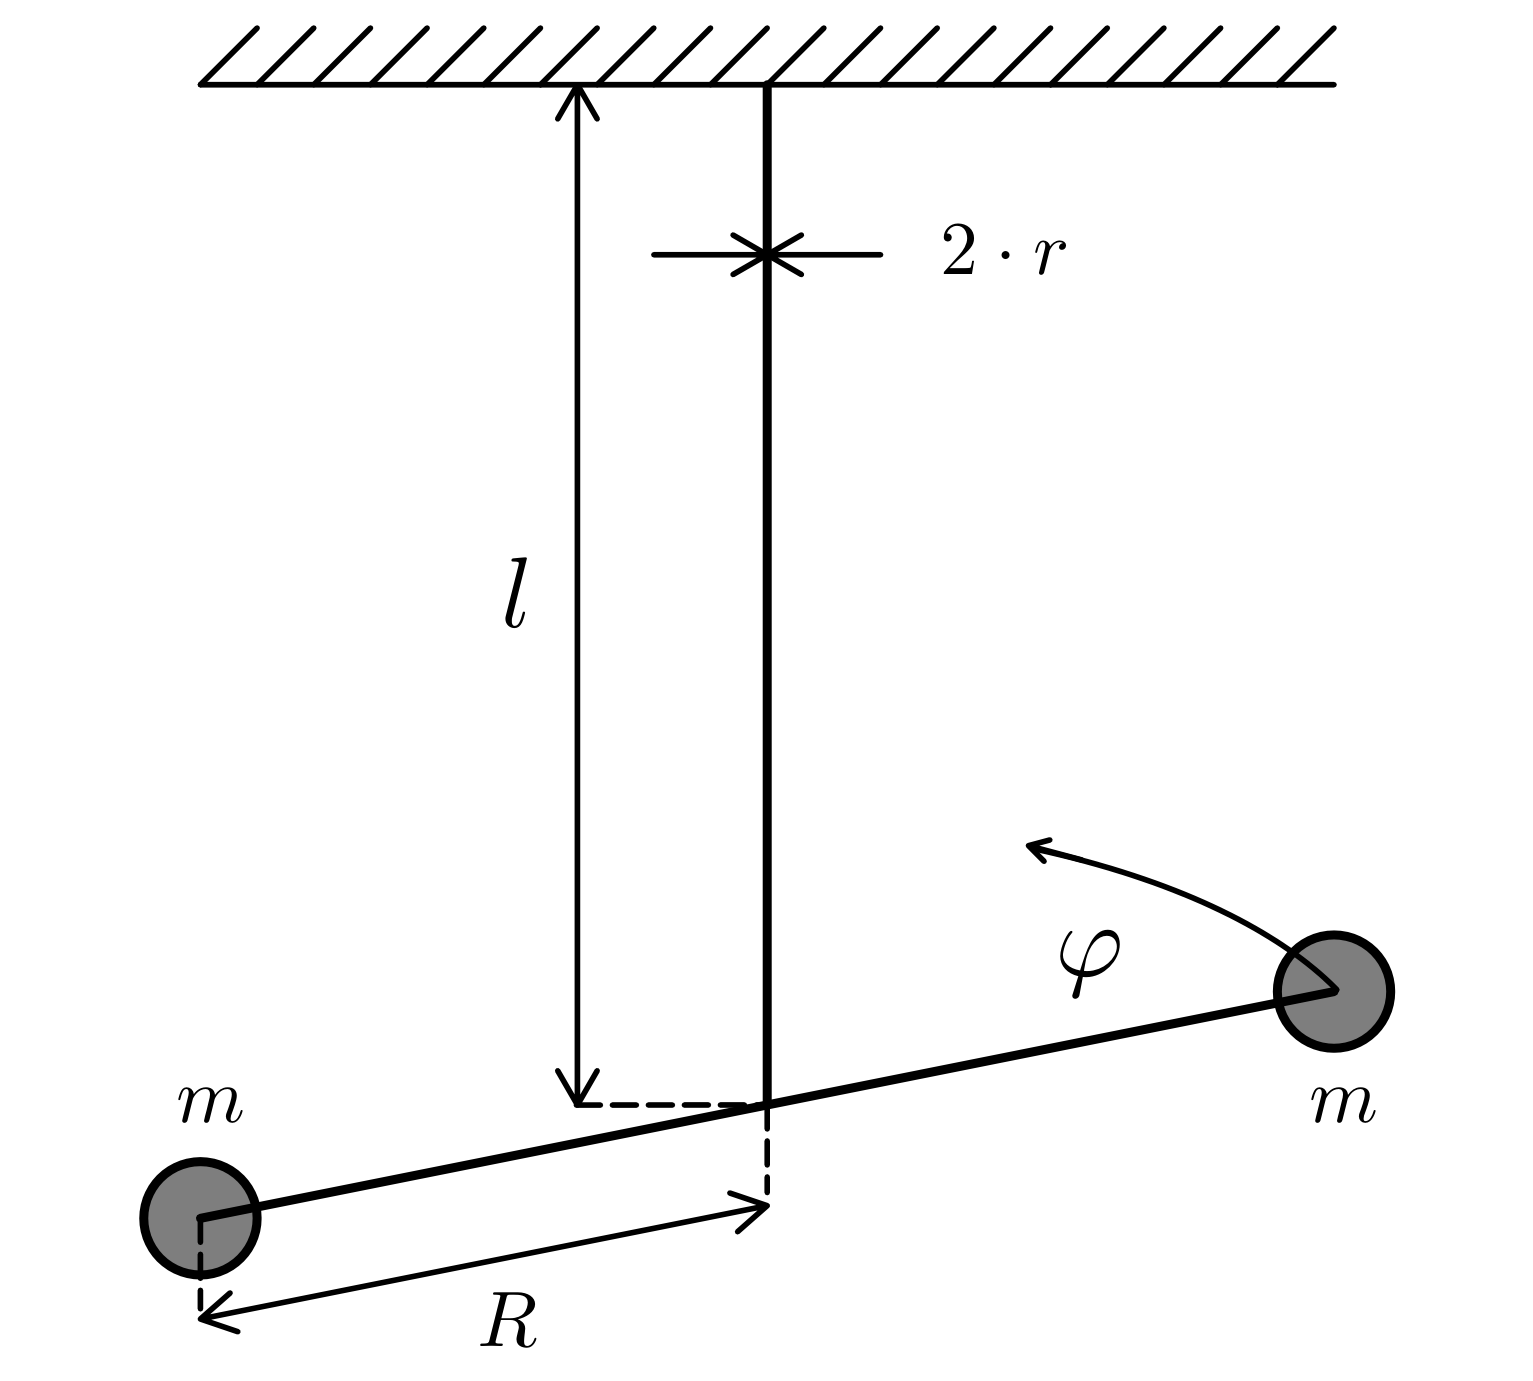
\includegraphics[width=0.6\textwidth]{plots/skizze.png}
    \caption{Skizze des Torsionspendels. \textsl{Zeichnen Sie hier eine sinvolle Skizze des Versuchsaufbaus und beschriften Sie diese inklusive aller Messpositionen und Konstanten.}}
    \label{fig:skizze}
\end{figure}

\subsection{Versuchsdurchführung}
Zuerst wurden die Abmessungen des Pendels sowie die für die Auswertung erforderlichen anderen Größen bestimmt (siehe Abb. \ref{fig:skizze}).
Außerdem wurden die Fehler für die einzelnen Messungen abgeschätzt.
Die Massen, die während der Versuchsdurchführung am Pendel angebracht wurden, wurden mit einer elektronischen Waage des Typs "`Kern CB12K1N"' gewogen.
Die Zeitmessung erfolgte mit einer elektronischen Stoppuhr des Typs "`Triple Timer"'.
Die Abmessungen des Pendels wurden mit einem Bandmaß bestimmt; für die Bestimmung des Durchmessers des Drahtes wurde eine Mikrometerschraube verwendet, deren Bezeichnung auf Grund von häufiger Benutzung nicht mehr erkennbar war. 

Bei der Durchführung wurde wie folgt vorgegangen: Zuerst wurde die Ruhelage des Pendels bestimmt. Von dort aus wurde dem Pendel eine Anfangsamplitude von einer Umdrehung gegeben.
Bei Starten des Pendels aus dieser Postion erfuhr es leichte vertikale Schwingungen um die horizontale Achse, welche über die Dauern der einzelnen Messungen bestehen blieben.
Die Zeitmessung erfolgte an demjenigen Umkehrpunkt der Pendelbewegung, bei dem die Pendelbewegung startete.

Der Messzeitraum am Pendel umfasste 30 Schwingungen bei der Massepositionierung am äußeren Rand des Pendels.
Bei den anderen Messungen wurde nur über einen Zeitraum von 25 Schwingungen gemessen, wobei versehentlich jeweils eine Schwingung zusätzlich gezählt und somit 26 Schwingungen aufgenommen wurden. Die Reduzierung der Schwingungsanzahl erfolgte aus Zeitgründen.
Aus demselben Grund wurden pro Positionierung der Massen nur zwei statt drei Messungen durchgeführt.

Während jeder Messung der Schwingungsdauern war zu beobachten, dass die Amplitude der Pendelbewegung über den Messzeitraum kontinuierlich abgenommen hat, sodass sie zum Ende einer jeden Messung um ca. 180$^\circ$ reduziert war.
Dies entspricht ca. 50\% der Startamplitude.

\subsection{Messwerte}
\textsl{Erstellen Sie hier eine Tabelle mit den Messwerten und den zugehörigen abgeschätzten Messfehlern.}

\begin{table}[ht]
    \centering
    \begin{tblr}{
        colspec=cc, rowsep=2pt,
        vlines{}, hline{1,2,3},    
        }
        Länge $l \;/\; \si{\meter}$ & Durchmesser $d \;/\; \si{\meter}$ \\
        \num{1,500(3)} & \num{5,0(2)e-4} \\
    \end{tblr}
    \caption{Gemessene Eigenschaften des Drahtes.}
    \label{tab:draht}
\end{table}
\begin{table}[ht]
    \centering
    \begin{tblr}{
        colspec=ccccc, rowsep=2pt,
        vlines{}, hline{1,2,4,8},
        cell{2}{2}={r=2}{c},
        cell{4}{2}={r=4}{c},
        cell{2}{3}={r=2}{c},
        cell{4}{3}={r=2}{c},
        cell{6}{3}={r=2}{c},
        }
        Messung & Masse $m \;/\; \si{\kilogram}$ & Position $R\;/\;\si{\meter}$ & $t \;/\; \si{\second}$ & \#Perioden n \\
        $t_{01}$ & -              &   -            & \num{755,53(100)} & 26 \\
        $t_{02}$ &                &                & \num{726,29(100)} & 25 \\
        $t_{11}$ & \num{0,393(1)} & \num{0,045(3)} & \num{806,59(100)} & 26 \\
        $t_{12}$ &                &                & \num{775,66(100)} & 25 \\
        $t_{21}$ &                & \num{0,200(3)} & \num{1637,8(10)}  & 30 \\
        $t_{22}$ &                &                & \num{1638,0(10)}  & 30 \\
    \end{tblr}
    \caption{Gemessene Zeiten der sechs Einzelmessungen.}
    \label{tab:messwerte}
\end{table}
